% Section content template for individual Educative lessons
% This file contains the actual content for a specific section
% Generated from Educative API section content

% Section: Requirements of a Blob Store's Design
% Section ID: 5129194917068800
% Section Slug: requirements-of-a-blob-stores-design
% Generated: 2025-12-07T21:36:44.907413

\subsection{Requirements}\label{OgrKwILwMEDGKQZ2UWGAM}
\\
Let's understand the functional and non-functional requirements below:

\subsubsection{Functional requirements}\label{_X5hhr6FLKMhdQaPeokfh}
\\
Here are the functional requirements of the design of a blob store:

\begin{itemize}
\item
\protect\phantomsection\label{c4k31iVnI5RqYhQE9Kf9u}
\textbf{Create a} \textbf{container}(A container is like a folder in a file system used to group blobs. Don't mix up this container with a Docker container.): The users should be able to create containers in order to group blobs. For example, if an application wants to store user-specific data, it should be able to store blobs for different user accounts in different containers. Additionally, a user may want to group video blobs and separate them from a group of image blobs. A single blob store user can create many containers, and each container can have many blobs, as shown in the following illustration. For the sake of simplicity, we assume that we can't create a container inside a container.
\end{itemize}

\begin{figure}[htbp]
 \centering
 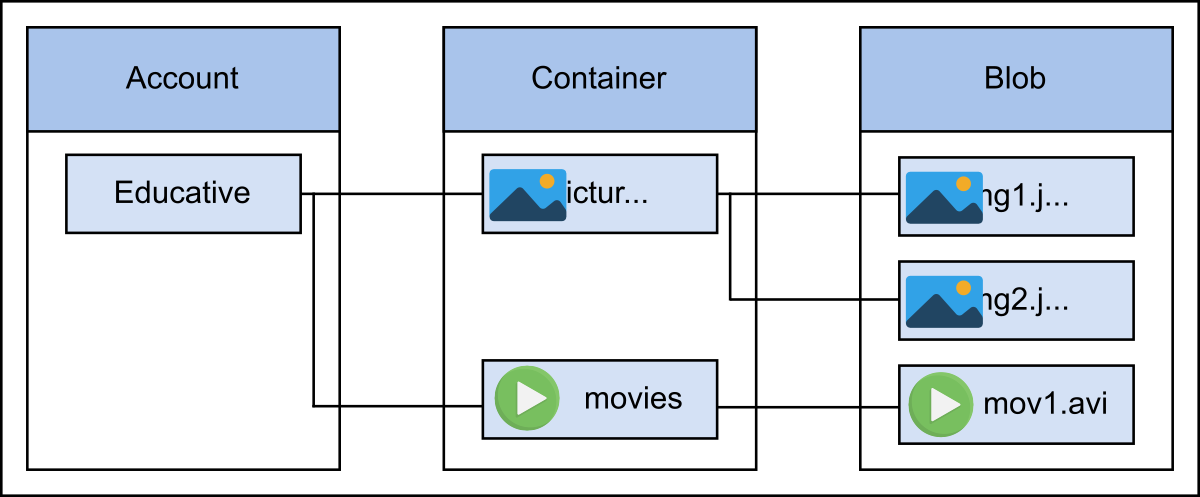
\includegraphics[width=0.5\textwidth]{Images/chapter_20/section_5129194917068800/6093599408521216.png}
 \caption{Multiple containers associated with a single storage account, and multiple blobs inside a single container}
\end{figure}

\begin{itemize}
\item
\protect\phantomsection\label{qH5eTqg0YQnQWL4c3o5He}
\textbf{Put data:} The blob store should allow users to upload blobs to the created containers.
\item
\protect\phantomsection\label{AvqF0Zn_i8ys8c_swZYXB}
\textbf{Get data:} The system should generate a URL for the uploaded blob, so that the user can access that blob later through this URL.
\item
\protect\phantomsection\label{f894Du4f6m62Kje0Cy2_h}
\textbf{Delete data:} The users should be able to delete a blob. If the user wants to keep the data for a specified period of time (retention time), our system should support this functionality.
\item
\protect\phantomsection\label{coWY5GWsfoO8b5f-14Krr}
\textbf{List blobs:} The user should be able to get a list of blobs inside a specific container.
\item
\protect\phantomsection\label{LBk3E1tjikjVJDHipqv_F}
\textbf{Delete a container:} The users should be able to delete a container and all the blobs inside it.
\item
\protect\phantomsection\label{F-3w2WVJuGu-F_8n5jszD}
\textbf{List containers:} The system should allow the users to list all the containers under a specific account.
\end{itemize}

\begin{figure}[htbp]
 \centering
 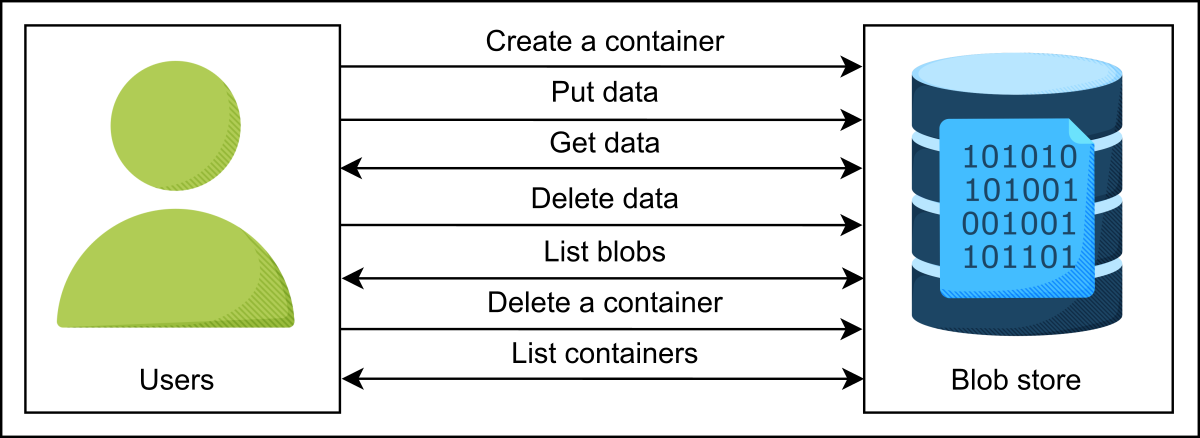
\includegraphics[width=0.5\textwidth]{Images/chapter_20/section_5129194917068800/6750341750456320.png}
 \caption{Functional requirements of a blob store}
\end{figure}

\subsubsection{Non-functional requirements}\label{guXWXSPYsdMGPDpRTFcx9}
\\
Here are the non-functional requirements of a blob store system:

\begin{itemize}
\item
\protect\phantomsection\label{MR3Q7jKil2z9s8iq_-4Lj}
\textbf{Availability:} Our system should be highly available.
\item
\protect\phantomsection\label{57s_HOMO8_QyfR7jeAWvy}
\textbf{Durability:} The data, once uploaded, shouldn't be lost unless users explicitly delete that data.
\item
\protect\phantomsection\label{PN4CDgTjjw6T0L4evkgIX}
\textbf{Scalability:} The system should be capable of handling billions of blobs.
\item
\protect\phantomsection\label{2i-tG4mVFKr0bJ_6gfnD7}
\textbf{Throughput}: For transferring gigabytes of data, we should ensure a high data throughput.
\item
\protect\phantomsection\label{XN0DJDa1hYDwtL81lkLVO}
\textbf{Reliability:} Since failures are a norm in distributed systems, our design should detect and recover from failures promptly.
\item
\protect\phantomsection\label{Kytv8mSF8z5s88y8rtrwM}
\textbf{Consistency:} The system should be strongly consistent. Different users should see the same view of a blob.
\end{itemize}

\begin{figure}[htbp]
 \centering
 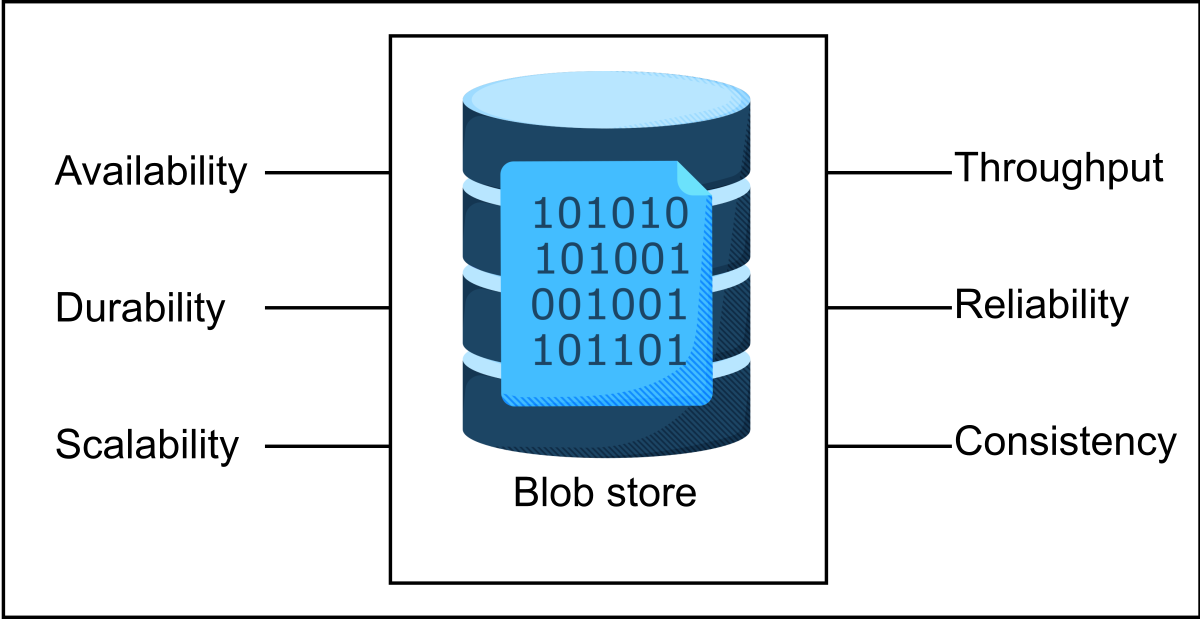
\includegraphics[width=0.5\textwidth]{Images/chapter_20/section_5129194917068800/5470099123601408.png}
 \caption{The non-functional requirements of a blob store}
\end{figure}

Explain the concept of eventual consistency in the context of blob stores. Provide a scenario where it might be acceptable in the widget below.


\subsection{Resource estimation}\label{h0U1_4HpwXCWjr4lUXH7t}
\\
Let's estimate the total number of servers, storage, and bandwidth required by a blob storage system. Because blobs can have all sorts of data, mentioning all of those types of data in our estimation may not be practical. Therefore, we'll use YouTube as an example, which stores videos and thumbnails on the blob store. Furthermore , we'll make the following assumptions to complete our estimations.
\\
\textbf{Assumptions:}

\begin{itemize}
\item
\protect\phantomsection\label{A--Q0EgFZ6C0W8dQImtx5}
The number of daily active users who upload or watch videos is five million.
\item
\protect\phantomsection\label{xiZYhMT2ZfDlyfYvBhdax}
The number of requests per second that a single blob store server can handle is 500(This number can be significantly higher, depending upon the blob store. For example, Microsoft Azure can handle a maximum of 20,000 IOPS.).
\item
\protect\phantomsection\label{VFciHqgyN897AuEYj5HFT}
The average size of a video is 50 MB.
\item
\protect\phantomsection\label{UKAVTad0xDxBdY4SgUsGT}
The average size of a thumbnail is 20 KB.
\item
\protect\phantomsection\label{FW7x2EogdONUvKeR92NZE}
The number of videos uploaded per day is 250,000.
\item
\protect\phantomsection\label{SbKcCZe-SKKvKRcRSPp2D}
The number of read requests by a single user per day is 20.
\end{itemize}

\subsubsection{Number of servers estimation}\label{SSa8aib22ogN3Dl7IBRs2}
\\
Considering \href{https://www.educative.io/courses/grokking-the-system-design-interview/put-back-of-the-envelope-numbers-in-perspective}{our assumption} of using~daily active users as a proxy for the number of requests per second for peak load times, we get 5 million requests per second. The number of servers that we require, considering 500 RPS for the blob store server, is calculated using the formula given below:

\[
\text{Servers needed at peak load} = \frac{\text{Number of requests/second}}{\text{RPS of server}}
\]

\[
\text{Servers needed at peak load} = \frac{5 \ \text{million}}{500} = \text{10K} \ \text{servers}
\]

\begin{figure}[htbp]
 \centering
 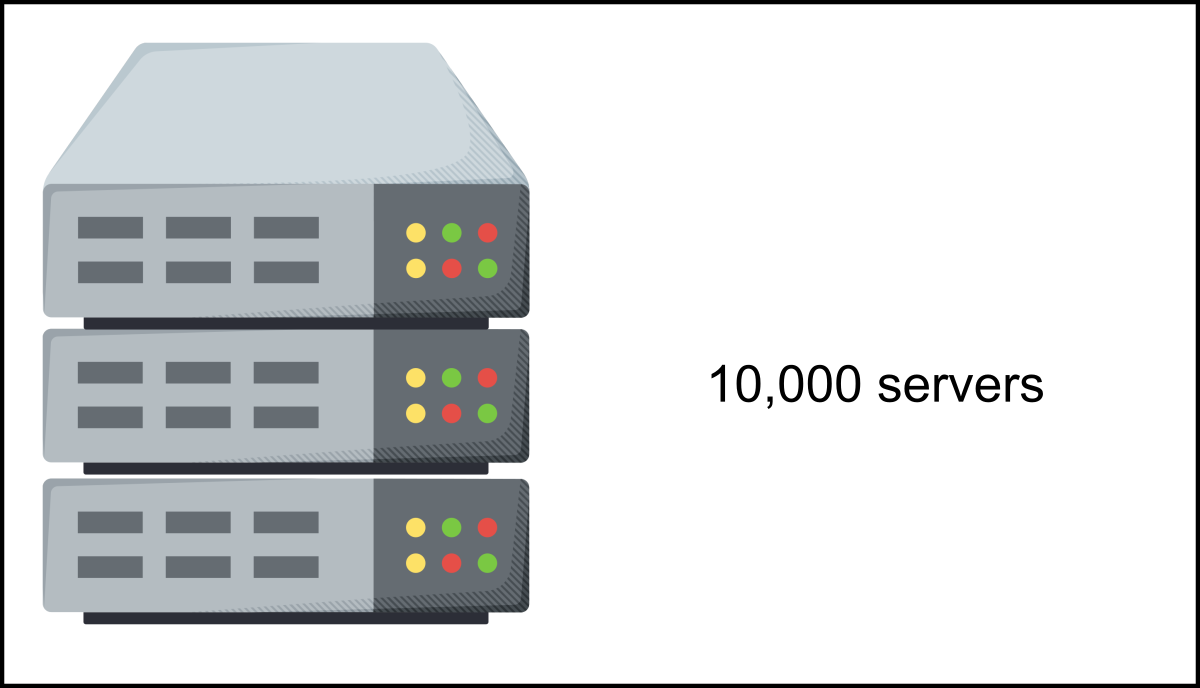
\includegraphics[width=0.25\textwidth]{Images/chapter_20/section_5129194917068800/5635793576394752.png}
 \caption{Number of servers required by a blob store system dedicated to storing YouTube data}
\end{figure}

\begin{quote}
\textbf{Note:} Our revised estimate for the blob store server is 500 RPS, down from 64,000 RPS, to accommodate the I/O-intensive nature of a blob store server, where operations typically take longer to execute.
\end{quote}
\subsubsection{Storage estimation}\label{1naUHazqZvwXbsXTORyKC}
\\
Considering the assumptions written above, we use the formula given below to compute the total storage required by YouTube in one day:

\[
\text{Total}_{\text{storage/day}} = \text{No. of videos}_{\text{/day}} \times \left( \text{Storage}_{\text{/video}} + \text{Storage}_{\text{/thumbnail}} \right)
\]

Putting the numbers from above into the formula gives us \protect\phantomsection\label{katex_inline_fu6-1xWDdgybbmLgdSekU}{{{\(12.51\ \text{TB}_{/ \text{day}}\)}}}, which is the approximate storage required by YouTube per day for keeping a single copy of the uploaded videos in a single resolution.

\begin{figure}[htbp]
 \centering
 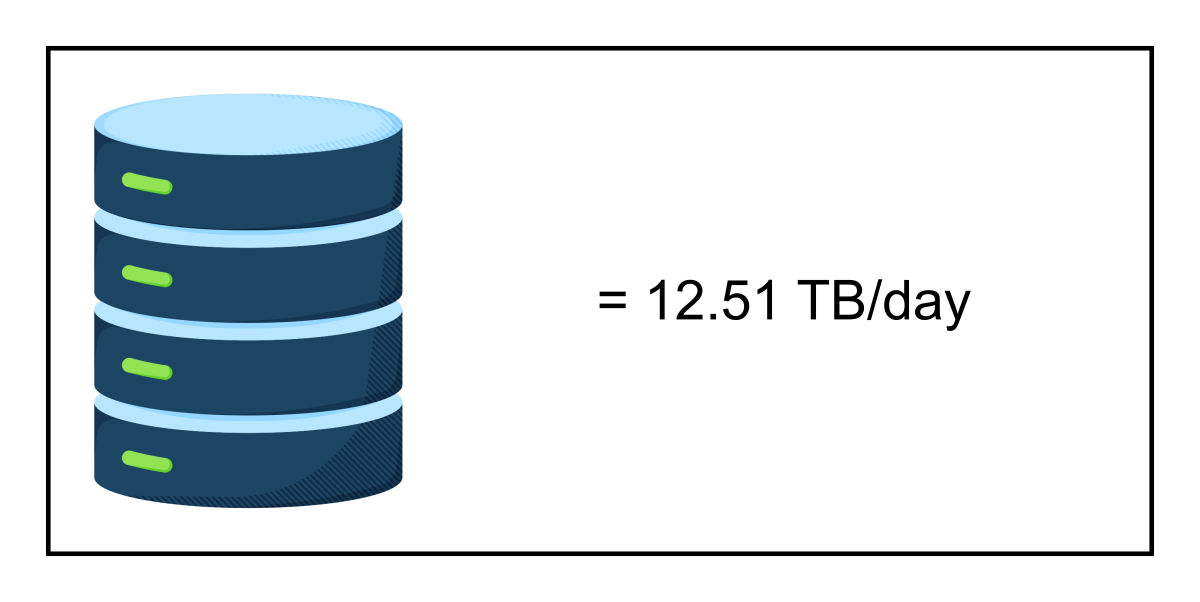
\includegraphics[width=0.25\textwidth]{Images/chapter_20/section_5129194917068800/5802415688122368.png}
 
\end{figure}

\subsubsection{Bandwidth estimation}\label{xn8qslLEmd0Bm-IIQqLqu}
\\
Let's estimate the bandwidth required for uploading data to and retrieving data from the blob store.
\\
\textbf{Incoming traffic}: To estimate the bandwidth required for incoming traffic, we consider the total data uploaded per day, which indirectly means the total storage needed per day that we calculated above. The amount of data transferred to the servers per second can be computed using the following formula:

\[
\text{Total}_{\text{bandwidth}} = \frac{\text{Total}_{\text{storage/day}}}{24 \times 60 \times 60}
\]

\textit{Component type 'InstaCalc' not yet supported.}

\textbf{Outgoing traffic}: Since the blob store is a read-intensive store, most of the bandwidth is required for outgoing traffic. Considering the aforementioned assumptions, we calculate the bandwidth required for outgoing traffic using the following formula:

\[
\text{Total}_{\text{bandwidth}} = \frac{\text{No. of active users}_{\text{/day}} \times \text{No. of requests}_{\text{/user/day}} \times \text{Total}_{\text{data size}}}{\text{Seconds in a day}}
\]

\textit{Component type 'InstaCalc' not yet supported.}

\begin{figure}[htbp]
 \centering
 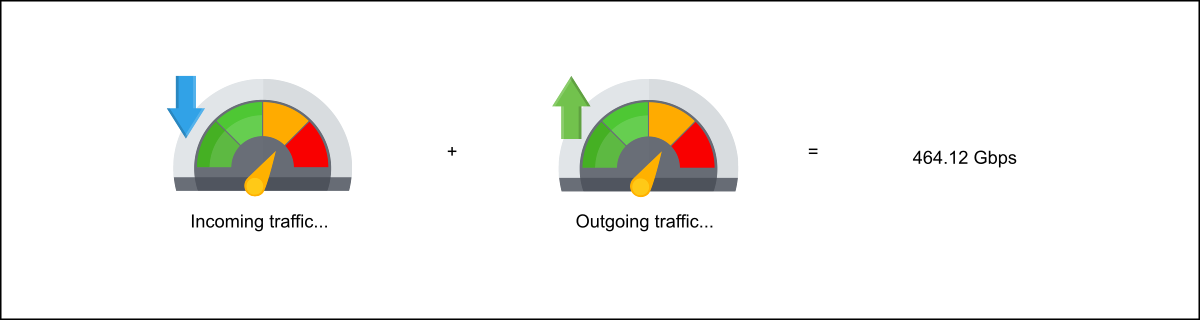
\includegraphics[width=0.5\textwidth]{Images/chapter_20/section_5129194917068800/5232055751540736.png}
 \caption{Summarizing the bandwidth requirements of a blob store system for YouTube videos only}
\end{figure}

\subsection{Building blocks we will use}\label{xhKKen_zdcnzKYs3KpTqO}
\\
We use the following building blocks in the design of our blob store system:\\
\strut \\

\begin{figure}[htbp]
 \centering
 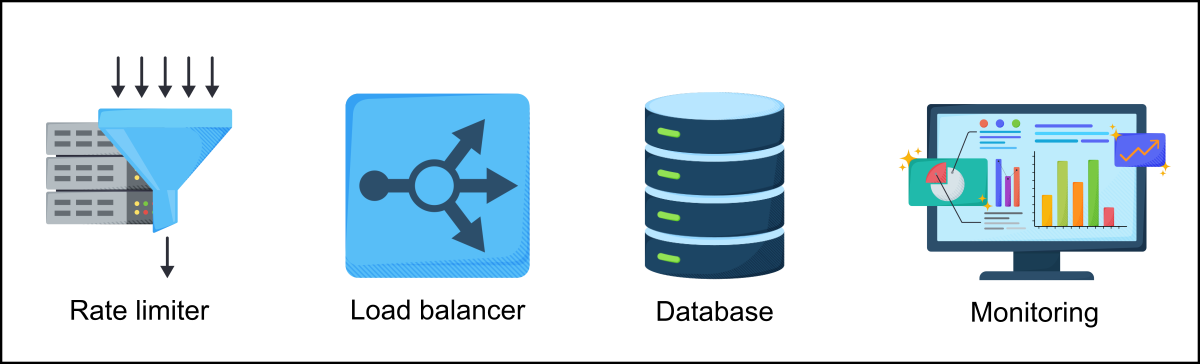
\includegraphics[width=0.5\textwidth]{Images/chapter_20/section_5129194917068800/5353114599555072.png}
 \caption{Building blocks for the design of a blob store}
\end{figure}

\begin{itemize}
\item
\protect\phantomsection\label{4gOeXJagJhUjMmZLIgg2B}
\href{https://www.educative.io/courses/grokking-the-system-design-interview/system-design-the-rate-limiter}{\textbf{Rate Limiter:}} A rate limiter is required to control the users' interaction with the system.
\item
\protect\phantomsection\label{8taOd18lZxXeqZfkafi-j}
\href{https://www.educative.io/courses/grokking-the-system-design-interview/introduction-to-load-balancers}{\textbf{Load balancer:}} A load balancer is needed to distribute the request load onto different servers.
\item
\protect\phantomsection\label{-2lxue25x6WiwMsiZCbXQ}
\href{https://www.educative.io/courses/grokking-the-system-design-interview/introduction-to-databases}{\textbf{Database:}} A database is used to store metadata information for the blobs.
\item
\protect\phantomsection\label{bQlgADz0svjdvVlRVY-1F}
\href{https://www.educative.io/courses/grokking-the-system-design-interview/system-design-distributed-monitoring}{\textbf{Monitoring:}} Monitoring is needed to inspect storage devices and the space available on them in order to add storage on time if needed.
\end{itemize}
\\
In this lesson, we discussed the requirements and estimations of the blob store system. We 'll design the blob store system in the next lesson, all while following the delineated requirements.

% End of section content